\section{Scaling Laws}

There are two main phases of a bubble bursting. First is an initial cavity collapse, creating a singularity. This singularity causes a jet to rapidly shoot upwards and possibly release droplets.

\begin{figure}[!h]
    \centering
    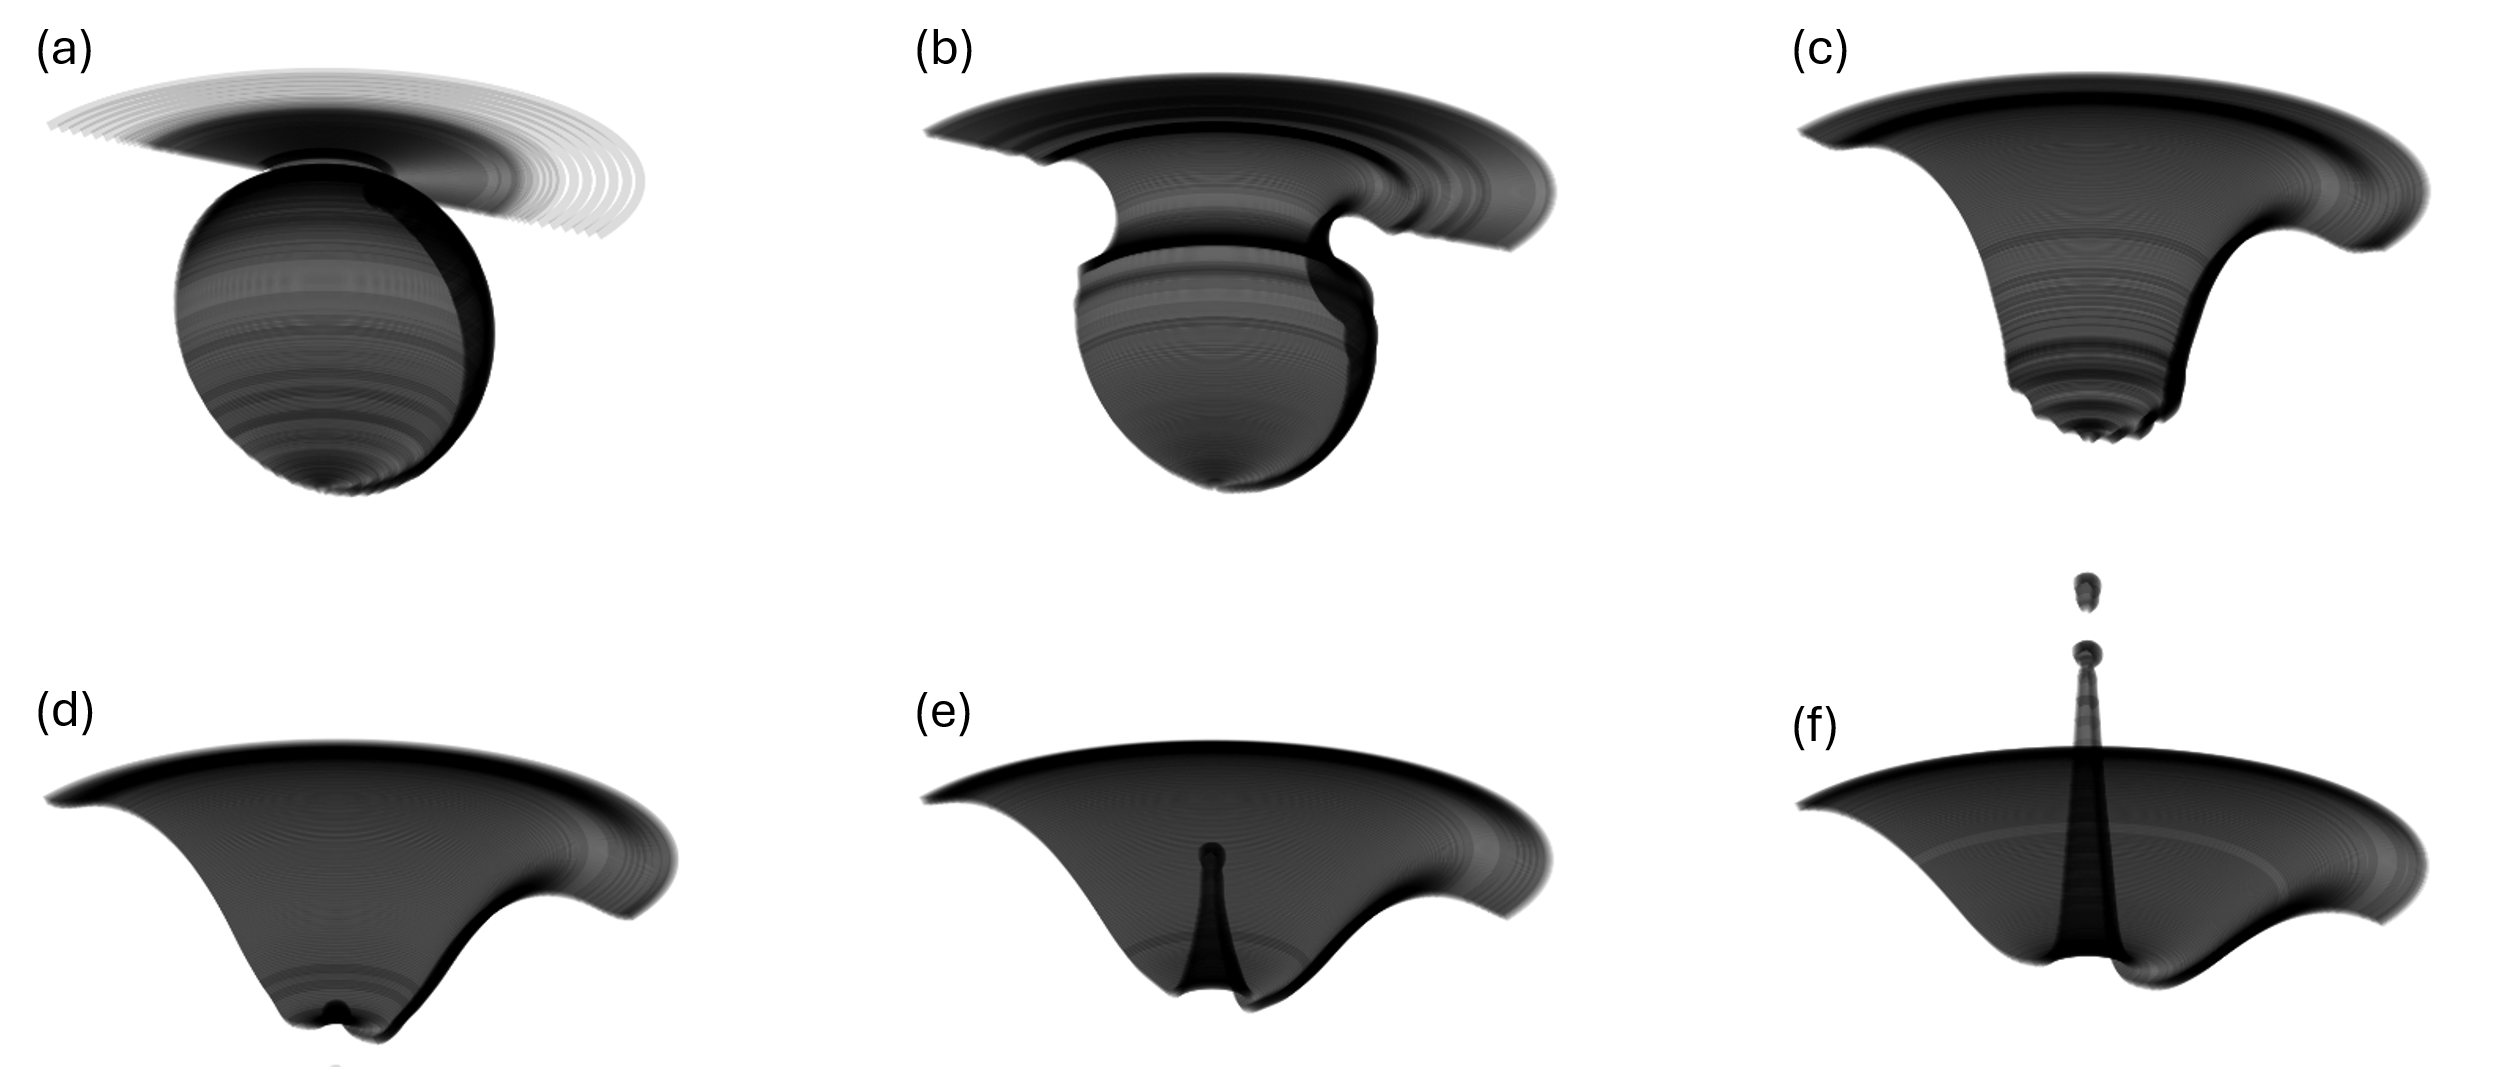
\includegraphics[width=0.8\linewidth]{WriteUp/images/many 3D profiles.png}
    \caption{Evolution of a bubble bursting. In figures (a)-(c) we see the cavity collapsing in on itself. In figures (e)-(f) we see the formation of the jet and in figure (f) we see the release of a droplet}
    \label{fig:Profiles}
\end{figure}

Recently, progress was made linking jet dynamics with the physical properties of the liquid. Ghabache \textit{et al.} \cite{ghabache2014physics} developed scaling laws for the jet velocity as a function of the size of the jet drop, the liquid properties and the initial size of the bubble. A set of scaling laws
for the jet velocity, as well as the radial and axial length of
the, jet as a function of the liquid properties, have been
developed using a force and energy argument \cite{ganan2017revision}. The
effects of gravity were investigated theoretically \cite{ganan2018scaling}. The
effect of gravity on jet velocity and the critical conditions
for ejection of jet drops were examined numerically by
Deike \textit{et al.} \cite{deike2018dynamics}.

Zeff \textit{et al.} \cite{zeff2000singularity} showed that a liquid-water interface is self-similar
and obeys inertial-capillary scaling law until a surface wave collapse at time $t_0$. This was done by first assuming the fluid is irrotational and incompressible, i.e.
\begin{align}
    &\nabla \cdot \textbf{u}=0&&\nabla \times \textbf{u}=0,
\end{align}
and that the air above the fluid is considered to be of zero density. near the singularity, the surface tension forces, kinetic energy density and acceleration are all thought to diverge and due to the small length scales gravity may safely be neglected. The system can then be described by three equations, one for the inside of the fluid and two for the fluid-air interface:

\begin{gather}\label{scaling euqations 1}
    \Delta\phi=0,\\ \label{scaling euqations 2}
    \frac{\partial h}{\partial t}+\frac{\partial h}{\partial r}\frac{\partial \phi}{\partial r}=\frac{\partial \phi}{\partial z},\\ \label{scaling euqations 3}
    \frac{\partial \phi}{\partial t} + \frac{1}{2}(\nabla \phi)^2 + \frac{\sigma}{\rho}\left( \frac{1}{R_1}+\frac{1}{R_2}\right),
\end{gather}
where $\phi$ is the velocity potential ($\textbf{u}=\nabla \phi$), $z$ is the axial coordinate ($z=h$ at the free surface), $r$ is the radial distance, $\sigma$ and $\rho$ are the surface tension and density of the fluid respectively and $R_1$ and $R_2$ are the principal radii of curvature of the surface. The first equations represents the incompressibility of the fluid and the second equation represents the kinematic boundary condition on the fluid surface and the last equation is the Bernoulli equation at the fluid surface, all in cylindrical coordinates.

They then postulate a power-law scaling in times close to the singularity:
\begin{gather}\label{postulated 1}
    h(r,t)=(t_0-t)^{\alpha}f[r(t_0-t)^{\beta}]\\ \label{postulated 2}
    \phi(r,z,t)=(t_0-t)^{\gamma}g[r(t_0-t)^{\beta},z(t_0-t)^{-\alpha}],
\end{gather}
where the variables $r$ and $z$ have been scaled by the characteristic length and velocity scales.

For a similarity solution to exist, the time-dependence of all terms in equations \ref{scaling euqations 1}\ref{scaling euqations 2}\ref{scaling euqations 3}. After substituting in the proposed power scalings they found only a single value is allowed for each exponent:
\begin{align}
    \alpha=\frac{2}{3}, &&\beta = -\frac{2}{3}, && \gamma=\frac{1}{3}
\end{align}
These exponents were also found by Keller and Miksis \cite{keller1983surface}. This scaling law only describes the dynamics up to the cavity collapse singularity.Lai \textit{et al.} showed that for both cavity collapse ($t<t_0$) and jet formation ($t>t_0$), the time-dependent profiles obey a $|t-t_0|^{2/3}$ inviscid scaling\cite{lai2018bubble}.